%%%%%%%%%%%%%%%%%%%%%%%%%%%%%%%%%%
\chapter{Revisão matemática}
\label{Chap:Review}
%%%%%%%%%%%%%%%%%%%%%%%%%%%%%%%%%%

%\minitoc

%\clearpage

%%%%%%%%%%%%%%%%%%%%
\section{Introdução}
%%%%%%%%%%%%%%%%%%%%

{\it
Precisamos calcular coisas. Algumas propriedades matemáticas importantes que serão utilizadas ao longo do curso são apresentadas abaixo.
}

%%%%%%%%%%%%%%%%%
\section{Frações}
%%%%%%%%%%%%%%%%%

%%%%%%%%%%%%%%%%%%%
\section{Potencias}
%%%%%%%%%%%%%%%%%%%

%%%%%%%%%%%%%%%%%%%%%%%%%%%%%%%%%%%%%%%%%
\section{Equações e sistemas de equações}
%%%%%%%%%%%%%%%%%%%%%%%%%%%%%%%%%%%%%%%%%

%%%%%%%%%%%%%%%%%
\section{Funções}
%%%%%%%%%%%%%%%%%

%%%%%%%%%%%%%%%%%%%
\section{Geometria}
%%%%%%%%%%%%%%%%%%%

% áreas e volumes

\begin{figure}
\centering
\begin{tikzpicture}

\path [draw, name path = horiz] (0,0) coordinate (start-horiz) -- (4,0) coordinate (end-horiz);
\path [draw, name path = trans] (1,-1) coordinate (start-trans) -- (3,1) coordinate (end-trans);

\path [name intersections={of = horiz and trans}] (intersection-1) coordinate (intersec);

\pic [draw, "$\alpha$", angle eccentricity=1.5] {angle = end-horiz--intersec--end-trans};
\pic [draw, "$\alpha$", angle eccentricity=1.5] {angle = start-horiz--intersec--start-trans};
\pic [draw, "$\beta$", angle eccentricity=1.5, angle radius = 3mm] {angle = start-trans--intersec--end-horiz};
\pic [draw, "$\beta$", angle eccentricity=1.5, angle radius = 3mm] {angle = end-trans--intersec--start-horiz};

\draw[fill] (start-horiz) node[left]{$A$} circle (0.5pt);
\draw[fill] (end-horiz) node[right]{$B$} circle (0.5pt);
\end{tikzpicture}
\caption{Os ângulos opostos pelo vértice (encontro das duas retas) são iguais.}
\end{figure}

\begin{figure}
\centering
\begin{tikzpicture}
\path[name path = sup, draw] (0,0) coordinate (start-sup) -- (4,0) coordinate (end-sup);
\path[name path = inf, draw] (0,-1.5) coordinate (start-inf) -- (4,-1.5) coordinate (end-inf);
\path[name path = trans, draw] (1, -2) coordinate (start-trans) -- (3, 0.5) coordinate (end-trans);

\draw[fill] (start-sup) node[left]{$A$} circle (0.5pt);
\draw[fill] (start-inf) node[left]{$C$} circle (0.5pt);
\draw[fill] (end-sup) node[right]{$B$} circle (0.5pt);
\draw[fill] (end-inf) node[right]{$D$} circle (0.5pt);

\path[name intersections={of= sup and trans}] (intersection-1) coordinate (int-sup);
\path[name intersections={of= inf and trans}] (intersection-1) coordinate (int-inf);

\pic[draw, "$\theta$", angle eccentricity=1.5]{angle = end-sup--int-sup--end-trans};
\pic[draw, "$\theta$", angle eccentricity=1.5]{angle = end-inf--int-inf--int-sup};

\end{tikzpicture}
\caption{Se as retas $\overline{AB}$ e $\overline{CD}$ são paralelas e uma reta transversal as atravessa, então os ângulos indicados na figura são necessariamente iguais.}
\end{figure}

\begin{figure}
\centering
\begin{tikzpicture}
\path[name path = sup, draw] (0,0) coordinate (start-sup) -- (4,0) coordinate (end-sup);
\path[name path = inf, draw] (0,-1.5) coordinate (start-inf) -- (4,-1.5) coordinate (end-inf);
\path[name path = trans, draw] (1, -2) coordinate (start-trans) -- (3, 0.5) coordinate (end-trans);

\draw[fill] (start-sup) node[left]{$A$} circle (0.5pt);
\draw[fill] (start-inf) node[left]{$C$} circle (0.5pt);
\draw[fill] (end-sup) node[right]{$B$} circle (0.5pt);
\draw[fill] (end-inf) node[right]{$D$} circle (0.5pt);

\path[name intersections={of= sup and trans}] (intersection-1) coordinate (int-sup);
\path[name intersections={of= inf and trans}] (intersection-1) coordinate (int-inf);

\pic[draw, "$\theta$", angle eccentricity=1.5]{angle = start-sup--int-sup--int-inf};
\pic[draw, "$\theta$", angle eccentricity=1.5]{angle = end-inf--int-inf--int-sup};

\end{tikzpicture}
\caption{Juntando os resultados anteriores, temos que os ângulos mostrados são iguais.\label{Fig:AlternosInternos}}
\end{figure}

\begin{figure}
\centering
\begin{tikzpicture}[scale = 1.2]
\draw[dashed] (0,0) coordinate (sup-starts) -- (3.5,0) coordinate (sup-ends);
\draw[dashed] (0,-1.5) coordinate (inf-starts) -- (3.5,-1.5) coordinate (inf-ends);
\draw (1,0) coordinate (A) -- (0.5,-1.5) coordinate (B) -- (3,-1.5) coordinate (C) -- cycle;

\pic[draw, "$\alpha$", angle eccentricity = 1.5] {angle = sup-starts--A--B};
\pic[draw, "$\alpha$", angle eccentricity = 1.5] {angle = C--B--A};

\pic[draw, "$\beta$", angle eccentricity = 1.5] {angle = C--A--sup-ends};
\pic[draw, "$\beta$", angle eccentricity = 1.5] {angle = A--C--B};

\pic[draw, "$\gamma$", angle eccentricity = 1.5, angle radius = 4mm] {angle = B--A--C};

\end{tikzpicture}
\caption{Note que na figura a soma dos ângulos na reta superior é \np[\tcdegree]{180}. Notamos também que, usando a Figura~\ref{Fig:AlternosInternos}, os ângulos internos inferiores do triângulo são iguais aos superiores externos. Logo, concluímos que a soma dos ângulos internos do triângulo também é \np[\tcdegree]{180}.}
\end{figure}

\paragraph{Teorema de Pitágoras}

Ao calcularmos a área total na Figura~\ref{Fig:TeoremaDePitagoras}, temos
\begin{align}
    A &= (a+b)^2 \\
    &= a^2 + b^2 + 2ab.
\end{align}
%
Também podemos determinar essa área através da soma da área do quadrado interno com a área dos quatro triângulos restantes:

\begin{align}
    A &= c^2 + 4 \frac{ab}{2} \\
    &= c^2 + 2ab.
\end{align}
\begin{marginfigure}[-4cm]
\centering
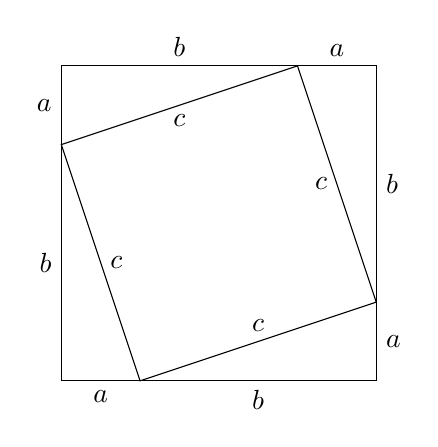
\begin{tikzpicture}
    \draw (0,0) rectangle (4,4);
    \draw (1,0) -- node[above]{$c$} (4,1) -- node[left]{$c$} (3,4) -- node[below]{$c$} (0,3) --node[right]{$c$} cycle;
    \node[below] (ad) at (0.5,0) {$a$};
    \node[right] (ar) at (4,0.5) {$a$};
    \node[above] (au) at (3.5, 4) {$a$};
    \node[left] (al) at (0, 3.5) {$a$};
    \node[below] (ad) at (2.5,0) {$b$};
    \node[right] (ar) at (4,2.5) {$b$};
    \node[above] (au) at (1.5, 4) {$b$};
    \node[left] (al) at (0, 1.5) {$b$};
\end{tikzpicture}
\caption{Através do cálculo da área chegamos no Teorema de Pitágoras. \label{Fig:TeoremaDePitagoras}}
\end{marginfigure}

\noindent{}Igualando as duas expressões para a área, temos
\begin{align}
    A &= A \\
    a^2 + b^2 + 2ab &= c^2 + 2ab \\
    a^2 + b^2 &= c^2 + 2ab - 2ab \\
    a^2 + b^2 &= c^2. \mathnote{Teorema de Pitágoras}
\end{align}


%%%%%%%%%%%%%%%%%%%%%%%
\section{Trigonometria}
%%%%%%%%%%%%%%%%%%%%%%%

%inclur o círculo trigonométrico nisso, além dos triângulos. mostrar a interpretação do seno, cosseno, tangente, cotangente, e o escambau

%%%%%%%%%%%%%%%%%%
\section{Gráficos}
%%%%%%%%%%%%%%%%%%

Explicar gráficos
